\begin{savequote}[8cm]
\textlatin{Neque porro quisquam est qui dolorem ipsum quia dolor sit amet, consectetur, adipisci velit...}

There is no one who loves pain itself, who seeks after it and wants to have it, simply because it is pain...
  \qauthor{--- Cicero's \textit{de Finibus Bonorum et Malorum}}
\end{savequote}

\chapter{\label{ch:35-nuint}Neutrino interactions} 
\minitoc
The underlying theory for neutrino oscillation is straightforward, and the parameters to be measured are clear, but the experimental determination of these parameters is challenging.
Due to the weak interaction of neutrinos, they cannot be detected directly.A
All neutrino measurements are based on the detection of the particles produced in the neutrino interaction.
Therefore, to extract the desired neutrino oscillation parameters with a high precision, a good understanding of neutrino interactions is crucial.
This chapter provides the basic understanding of neutrino interactions necessary for the interpretation of the analyses presented in the subsequent chapters.

\section{nu-quark}
The most fundamental interaction between a neutrino and matter is the weak interactions between the neutrino and a quark, the Feynman diagrams for which are shown in Fig.~\ref{fig:nu-q-feyn}.

\begin{figure}[h]
  \centering
  \begin{subfigure}[b]{0.45\textwidth}
    \centering
    \begin{tikzpicture}
      \begin{feynman}
        \vertex (a) {\(\nu_\ell\)};
        \vertex [right=of a] (b);
        \vertex [right=of b] (c) {\(\ell\)};
        \vertex [below=of b] (d);
        \vertex [left=of d] (e) {\(q\)};
        \vertex [right=of d] (f) {\(q'\)};
        
        \diagram* {
          (a) -- [fermion] (b) -- [fermion] (c),
          (b) -- [boson, edge label=\(W\)] (d),
          (e) -- [fermion] (d) -- [fermion] (f),
        };
      \end{feynman}
    \end{tikzpicture}
    \caption{Charge current interaction.}
    \label{fig:cc-interaction}
  \end{subfigure}
  \hfill
  \begin{subfigure}[b]{0.45\textwidth}
    \centering
    \begin{tikzpicture}
      \begin{feynman}
        \vertex (a) {\(\nu_\ell\)};
        \vertex [right=of a] (b);
        \vertex [right=of b] (c) {\(\nu_\ell\)};
        \vertex [below=of b] (d);
        \vertex [left=of d] (e) {\(q\)};
        \vertex [right=of d] (f) {\(q\)};
        
        \diagram* {
          (a) -- [fermion] (b) -- [fermion] (c),
          (b) -- [boson, edge label=\(Z\)] (d),
          (e) -- [fermion] (d) -- [fermion] (f),
        };
      \end{feynman}
    \end{tikzpicture}
    \caption{Neutral current interaction.}
    \label{fig:nc-interaction}
  \end{subfigure}
  \caption{Feynman diagrams for neutrino interactions with a quark.}
  \label{fig:nu-q-feyn}
\end{figure}
More specifically, Fig.~\ref{fig:cc-interaction} is mediated by the $W$ boson and the neutrino is converted to a charged lepton, while Fig.~\ref{fig:nc-interaction} is mediated by the $Z$ boson and the neutrino remains a neutrino.
The former is the charged current (CC) interaction, while the latter is the neutral current (NC) interaction.
Following the Feynman diagram, it is straightforward to write down the amplitude for the interaction.
The amplitude for the CC interaction is given by:
\begin{equation}
  \mathcal{M}_{\text{CC}} = \frac{g^2}{2} \bar{u}_\ell(p') \gamma^\mu (1 - \gamma^5) u_\nu(p) \frac{-i g_{\mu\nu}}{q^2 - M_W^2} \bar{u}_q(k') \gamma^\nu (1 - \gamma^5) u_q(k),
\end{equation}
where $g$ is the weak coupling constant, $u_\ell$ and $u_\nu$ are the spinors for the outgoing lepton and incoming neutrino, respectively, $u_q$ are the spinors for the quarks, $q$ is the momentum transfer, and $M_W$ is the mass of the $W$ boson.
This interaction takes place only when the neutrino possesses high enough energy <how high?> to probe inside the nucleon and interact with the quarks.
The product quark will hadronize and produce a jet of particles.
This type of interaction is refered to as deep inelastic scattering (DIS).
DIS is highly complicated, but no so relevant for this thesis, so will not be discussed further.
More details can be found in reviews, such as Ref.~\cite{}. <DIS review>

\section{nu-nucleon}
At the T2K beam energy, the predominant fraction of the neutrinos do not possess the energy to probe inside the nucleon, but rather interact with the nucleon as a whole.
Depending on the specific neutrino energy, the interaction can be classified as quasi-elastic (QE), resonance, or deep inelastic scattering (DIS).

  \subsection{QE}
  Although at the quark level, the interaction appears to the same as the $\nu$-quark interaction shown in Fig.~\ref{fig:nu-q-feyn}, the interacted quark cannot be treated as independent, but rather as part of a nucleon.
  Hence, the effective $\nu$-nucleon interaction feynman diagram is shown in Fig.~\ref{fig:nu-n-feyn}.
  \begin{figure}[h]
    \centering
    \begin{subfigure}[b]{0.45\textwidth}
      \centering
      \begin{tikzpicture}
        \begin{feynman}
          \vertex (a) {\(\nu_\ell\)};
          \vertex [right=of a] (b);
          \vertex [right=of b] (c) {\(\ell\)};
          \vertex [below=of b] (d);
          \vertex [left=of d] (e) {\(N\)};
          \vertex [right=of d] (f) {\(N'\)};
          
          \diagram* {
            (a) -- [fermion] (b) -- [fermion] (c),
            (b) -- [boson, edge label=\(W\)] (d),
            (e) -- [fermion] (d) -- [fermion] (f),
          };
        \end{feynman}
      \end{tikzpicture}
      \caption{Charge current interaction.}
      \label{fig:cc-interaction-n}
    \end{subfigure}
    \hfill
    \begin{subfigure}[b]{0.45\textwidth}
      \centering
      \begin{tikzpicture}
        \begin{feynman}
          \vertex (a) {\(\nu_\ell\)};
          \vertex [right=of a] (b);
          \vertex [right=of b] (c) {\(\nu_\ell\)};
          \vertex [below=of b] (d);
          \vertex [left=of d] (e) {\(N\)};
          \vertex [right=of d] (f) {\(N\)};
          
          \diagram* {
            (a) -- [fermion] (b) -- [fermion] (c),
            (b) -- [boson, edge label=\(Z\)] (d),
            (e) -- [fermion] (d) -- [fermion] (f),
          };
        \end{feynman}
      \end{tikzpicture}
      \caption{Neutral current interaction.}
      \label{fig:nc-interaction-n}
    \end{subfigure}
    \caption{Feynman diagrams for neutrino interactions with a nucleon.}
    \label{fig:nu-n-feyn}
  \end{figure}
  The leptonic current remains the same, but the hadronic current is now a nucleon current instead of a quark current.
  Hence, the hadronic current is much more complicated and and comprises of several form factors, which paramterize our understanding of the nucleon structure.
  For instance, the hadronic current for the CC interaction is given by:
  \begin{equation}
    \mathcal{M}_{\text{CC}} = \frac{G_F}{\sqrt{2}} \bar{u}_\ell(p') \gamma^\mu (1 - \gamma^5) u_\nu(p) \bar{u}_N(k') \left[ F_1(q^2) \gamma_\mu + F_2(q^2) \frac{i \sigma_{\mu\nu} q^\nu}{2M} + F_A(q^2) \gamma_\mu \gamma^5 + F_P(q^2) \frac{q_\mu \gamma^5}{m_\pi} \right] u_N(k),
  \end{equation}
  where $G_F$ is the Fermi constant, $F_1$, $F_2$, $F_A$, and $F_P$ are the form factors, $M$ is the nucleon mass, and $m_\pi$ is the pion mass.
  The derivation is complicated and beyond the scope of this thesis. 
  More details can be found in Ref.~\cite{LlewellynSmith:1978te}.
  It is however important to note that $F_1$ and $F_2$ are the vector form factors, which can be extracted from the electron scattering measurements, and $F_P$ is the pseudoscalar form factor, which can be related to $F_A$, the axial form factor, through the Partially Conserved Axial Current Hypothesis (PCAC) .
  Hence, the axial form factor is unique to neutrion experiments and can only be extracted from past measurements.

  \subsection{Resonance}
  When the neutrino energy is high enough to excite the nucleon to a higher energy state, e.g. $\Delta(1232)$ the interaction is classified as a resonance interaction.
  The excited nucleon then decays to produce a pion. 
  Hence, the resonance modelling is sometimes used interchangeably with the single pion production modelling.
  One of the most common moodel used today is the Berger-Sehgal model, which improves from the earlier Rein-Sehgal model by taking into account the effect of the lepton mass. (CHECK)
  The Rein-Sehgal model is based on the approximate relativistic quark model in Ref.~\cite{Feynman:1971wr}.
  Subsequent developments such as the MK model~\cite{Kabirnezhad:2017jmf,Kabirnezhad:2020wtp,Kabirnezhad:2022znc}, provides more sophisticated calculations.


\section{nu-nucleus}
Modern day neutrino experiments employ heavier elements, such as hydrocarbon and argon, to increase event rates.
This further complicates the neutrino interaction.
The simplest case is for the relatively high energy neutrino, for which the Impulse Approximation (IA) can be used.
The neutrino sees the nucleon as independent from other nucleons, so the interaction approaches the $\nu$-N interaction.
Even in this simplest case, the presence of the nuclear medium still affects the interaction in two ways, namely the intial state (IS) effect and the final state interaction (FSI).

When the neutrino energy drops, IA is no longer valid and can only resolve the nucleus as a whole.
In this case, Random Phase Approximation (RPA) correction is needed, which is beyond the scope of this thesis and will not be ellaborated further. 
Interest readers can refer to REFXXX for more details.
Instead, the two nuclear effects will be elaborated further below.

  \subsection{Initial state}
  The nuclear effects manifest in two ways.
  Firstly, the nucleon in the interaction is in a bound state, i.e. it cannot have arbitrary energy and momentum like a free nucleon.
  Instead, the energy distribution of the nucleon is parameterised by the so-called Spectral Function (SF).
  The simplest form of SF is the Fermi Gas model, which treats the nucleons as freely moving Fermi gas.
  Hence, the nucleon momentum is filled up to the Fermi momentum, which is given as:
  <CHECK>
  \begin{equation}
      k_F = (3\pi^2 \rho/2)^{1/3},
  \end{equation}
  where $\rho$ is the nuclear density.
  <How is the fermi momentum determined?>
  This model oversimplifies the nuclear structure.
  A more realistic model is the local Fermi gas (LFG) model, which accounts for the varying nuclear density, leading to an SF of the form:
  (CHECK)
  \begin{equation}
      S(k, E) = \int \rho(\vec{r}) \delta(E - \sqrt{k^2 + m^2}) d^3r,
  \end{equation}
  where $m$ is the nucleon mass.

  Further improvement, such as the short-range correlation between nucleons that increases the high momentum fraction.
  There are also effective SFs. Fit to data?

  \subsection{FSI}
  \label{sec:nuint-fsi}
  The second nuclear effect is the Final State Interaction (FSI).
  Regardless of how the neutrino interacts with the nucleon, the interaction products are still inside the nucleus.
  They have to propagate through the nuclear medium to be detectable.
  The interactions with the nuclear medium are classified as FSI.
  They are more pronounced for hadrons than leptons, as the former are more likely to interact with the nuclear medium.
  There are several types of FSI, such as the elastic scattering, charge exchange, and absorption.
  \begin{enumerate}
      \item 
  CEX involves changing the charge of the participating particles; for example,
  \begin{equation}
      \pip + \n \rightarrow \piz + \p,
  \end{equation}
  or vice versa. This rescattering type is crucial for event topologies requiring the presence of a pion;  depending on the signal pion charge, CEX could migrate events between signal and background. 

  \item 
  INEL is the case where the nucleus is left in an excited state after the rescattering. This category only contains the situation where a single additional nucleon is emitted/knocked-out after rescattering. Since it does not affect the number of pions produced, it will not convert an event from a pionless topology to a pion-production topology. The effects on nucleons are two-fold. Firstly, it can alter the number of signal events within each event topology. If the inelastic rescattering leads to two low-momentum protons below the detection threshold as opposed to a high-momentum proton, this signal event will be discarded as no protons are observed. Secondly, INEL invariably changes the kinematics of the rescattering particle. Be it the leading proton or the leading pion, based on which the TKI observables are calculated, the TKI distribution shape will be affected. Hence, while $\ninel$ would affect all four data sets, $\piinel$ would only affect \ttkpip and \minpiz. 

  \item 
  ABS refers to the case where the particle undergoes an interaction so that it does not emerge as a final particle. For example, $\pi^+$ can interact with two or more nucleons, initially forming a baryon resonance that subsequently interacts with other nucleons, emitting multiple nucleons rather than pions. Hence, the $\pi^+$ would not emerge from the nucleus anymore.

  \item 
  PIPD happens for energetic particles where an extra pion emerges as a result of the rescattering, such as
  \begin{equation}
      \p + \p \rightarrow \p + \n + \pip.
  \end{equation}
  Such an interaction significantly alters the event topology. 

  \end{enumerate}


\section{TKI}
\label{sec:nuint-tki}
Due to the heavy target nucleus in present neutrino experiments, nuclear effects are almost inextricable for conventional single particle kinematic measurement.
This highly impeds model development, as nuclear effects can micmic different $\nu$-N processes.
For instance, if the proton produced from a QE $\nu$-N interaction has high enough energy to produce an additional pion during FSI, which propagates out of the nucleus.
This QE event will micmic the output of a resonance interaction, or in term of topology, this CC$0\pi$ event will micmic a CC$1\pi$ event.
Hence, nuclear effects such as pion production can alter cross section measurements of different topologies differently, thereby impacting the modelling of the main underlying $\nu$-N interaction processes.
Therefore, an accurate description of the nuclear effect is crucial for reducing model systematics.
To gain insights on nuclear effects, observables that are particularly sensitive to these effects are indispensable. 
The Transverse Kinematic Imbalance (TKI) varaibles are exactly one such set of observables~\cite{Lu:2015hea, Lu:2015tcr}.
The TKI variables are shown in Fig.~\ref{fig:stki}.
\begin{figure}[!htb] 	
    \centering 		
    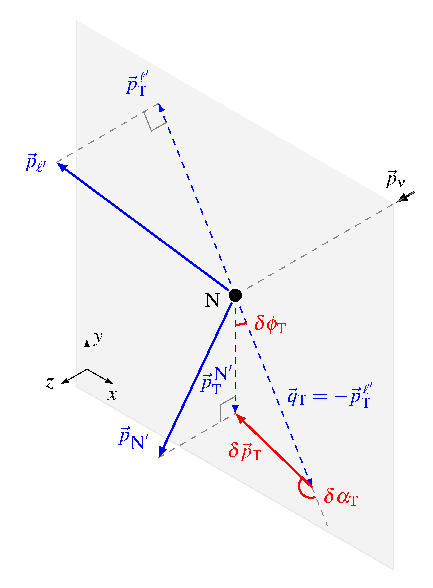
\includegraphics[width=0.35\textwidth]{figures/stki.eps}
    \caption{\label{fig:stki} Schematic illustration of the TKI variables. Diagram taken from Ref.~\cite{Lu:2015tcr}.} 
\end{figure}
In the simplest case, there are only two final particles after the neutrino-nucleon interaction, a muon and a proton. 
In the absence of nuclear effects, the muon and the proton should be emitted with momenta of the same magnitude but opposite direction in the plane transverse to the neutrino direction.
The TKI variables are constructed to quantify the deviation from this ideal scenario in measurements to access the nuclear effects. 
The presence of IS will affect the initial nucleon momentum, so the sum of the muon and proton transverse momenta will deviate from zero, which is quantified by $\dpt$, and their direction will not be exactly opposite, which is quantified by $\dphit$.
Furthermore, if the nucleus is assumed to be at rest and no other particles are knocked out other than the muon and the proton, the initial nucleon momentum, $\pn$, can also be estimated following the steps outlined in Ref.~\cite{Furmanski:2016wqo, Lu:2019nmf}. 
This esimation amounts to an approxiate  $\mathcal{O}(20\%)$ correction~\cite{Yang:2023dxk}. 
Hence, $\dpt$ and $\pn$ serve as good probes for IS models.
FSI will smear these distributions, but the shape and the peak position is mostly due to IS modelling.
All current IS models do not have a preferential direction for initial nuclear motion, so it is natural to assume the nucleons move in random directions isotropically, leading to a uniform $\dat$ distribution, which is the angle between the initial nucleon momentum and the proton momentum in the tranvserse plane. 
Thus, the deviation from flatness for $\dat$ can only be due to FSI, thereby making it an excellent probe for FSI. 
 
In the case of pion production, an additional doouble transverse variable, $\dptt$, can be constructed by projecting $\vecdpt$ onto the direction perpendicular to the lepton scattering plane, which is defined as the plane containing $\vecpl$ and $\vecpnu$.
The reconstruction is illustrated in Fig.~\ref{fig:dtki}.
\begin{figure}
    \centering
    \includegraphics[width=0.35\textwidth]{figures/dptt.pdf}
    \caption{\label{fig:dtki} Schematic illustration of the double TKI variable, $\dptt$. Diagram taken from Ref.~\cite{T2K:2021naz}.}
\end{figure}
In the absence of nuclear effects, $\dptt$ should be zero.
The spread of the $\dptt$ distribution is sensitive to the nuclear effects in pion production~\cite{MINERvA:2020anu, T2K:2021naz}.
Its equivalent in pionless production, $\dptx$, has been proposed and studied together with its orthogonal companion, $\dpty$, in MINERvA~\cite{MINERvA:2019ope}.
Additionally, Ref.~\ref{Lu:2015tcr,Hamacher-Baumann:2020ogq} suggests the possibility of using $\dptt$ to select a $\nu$-H sample.
Further details on a hydrogen sample selection will be discussed in Sec.~\ref{sec:tki-h}.

There has been a wealth of measurements from various neutrino experiments such as  T2K~\cite{T2K:2018rnz, T2K:2021naz}, MINERvA~\cite{MINERvA:2018hba, MINERvA:2019ope, MINERvA:2020anu, MINERvA:2021csy}, and MicroBooNE~\cite{MicroBooNE:2022emb, MicroBooNE:2023cmw, MicroBooNE:2023tzj, MicroBooNE:2023wzy, MicroBooNE:2024tmp}.
As the TKI idea is equally applicable to electron scattering, experiments such as CLAS~\cite{CLAS:2021neh} has also produced TKI measurments, showcasing the efficacy and wide applicability of TKI. 
